\chapter{Results}
\label{chapter:results}

We now present three experiments whose overarching goal is to evaluate our method and show results that cannot be achieved with conventional per-pixel projection mapping. Each section in this chapter corresponds to one experiment and is structured into three parts: 

\begin{itemize}
    \item Introduction which explains the goal and the setup of the experiment
    \item Results
    \item Analysis
\end{itemize}

We mostly provide a subjective analysis of our results because we have no metric that would determine how similar two textures look apart from the texture model itself that is used to generate the results. Visual inspection is thus our main method of analysis.

\section{Evaluating the basic idea of statistics-based projection mapping}
\label{section:results-experiments-01}

The basic idea of our proposed method is that when projecting a texture, instead of mapping it directly we use a texture synthesis algorithm to generate another realization of the same texture which is easier to map than the original texture. This process is superior to conventional per-pixel projection mapping of textures if the following assumptions hold:

\begin{itemize}
    \item Our texture model is sufficiently powerful
    \item Our algorithm is able to generate textures that both respect the model and are easy to map
\end{itemize}

In this experiment, we explore the second point.

\textbf{Goal.} The goal is to find out whether our method is indeed able to push the synthesis algorithm to generate textures that map well onto a given scene.

\textbf{Setup.} In our pipeline, we use the simple rendering function (see~\ref{section:methods-rendering_function-simple}) because it is sufficient for reproducing the conditions of our experiment. We also use the original unmodified Gatys texture model (see~\ref{section:methods-texture_model}) because we are not interested in overall performance, but simply whether it is possible to add restrictions to the texture model to make it generate only textures that match the background. The inputs to this experiment are pairs of scene (represented by a background image) and texture image \(\bm{y}\) that we wish to map onto the scene. The background is a subset of the texture image.

\begin{figure}[]
    \centering    
    \begin{subfigure}{\textwidth}
        \centering
        \begin{subfigure}{0.24\textwidth}
            \centering
            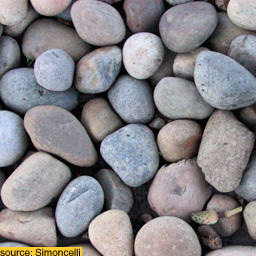
\includegraphics[width=\textwidth]{images/04-experiment01/pebbles/target.jpg}
            \caption{Desired appearance \(\bm{y}\)}
            \label{fig:ex01-pebbles-1000steps-some_target}
        \end{subfigure}
        \hfill
        \begin{subfigure}{0.24\textwidth}
            \centering
            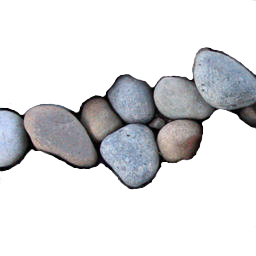
\includegraphics[width=\textwidth]{images/04-experiment01/pebbles/some_bg.jpg}
            \caption{Background}
            \vspace*{5mm}
            \label{fig:ex01-pebbles-1000steps-some_bg}
        \end{subfigure}
        \hfill
        \begin{subfigure}{0.24\textwidth}
            \centering
            \begin{tikzpicture}
                \draw (0, 0) node[inner sep=0] {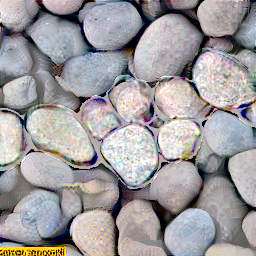
\includegraphics[width=\textwidth]{images/04-experiment01/pebbles/1000/some_im.jpg}};
                \fill[black] (-1.55, 1.0) rectangle ++(2.6, 0.6);
                \node [anchor=center] at (-0.25, 1.3) {{\color{white} Ours (Gatys)}};
            \end{tikzpicture}
            \caption{Compensated projection image \(\bm{p}\)}
            \label{fig:ex01-pebbles-1000steps-some_im}
        \end{subfigure}
        \hfill
        \begin{subfigure}{0.24\textwidth}
            \centering
            \begin{tikzpicture}
                \draw (0, 0) node[inner sep=0] {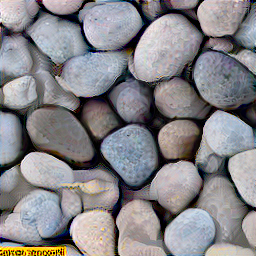
\includegraphics[width=\textwidth]{images/04-experiment01/pebbles/1000/some_proj.jpg}};
                \fill[black] (-1.55, 1.0) rectangle ++(2.6, 0.6);
                \node [anchor=center] at (-0.25, 1.3) {{\color{white} Ours (Gatys)}};
            \end{tikzpicture}
            \caption{Final appearance \(r(\bm{p})\)}
            \label{fig:ex01-pebbles-1000steps-some_proj}
        \end{subfigure}
        
        \begin{subfigure}{0.24\textwidth}
            \centering
            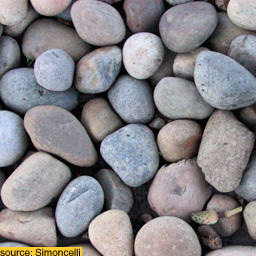
\includegraphics[width=\textwidth]{images/04-experiment01/pebbles/target.jpg}
            \caption{Desired appearance \(\bm{y}\)}
            \label{fig:ex01-pebbles-1000steps-threshold_target}
        \end{subfigure}
        \hfill
        \begin{subfigure}{0.24\textwidth}
            \centering
            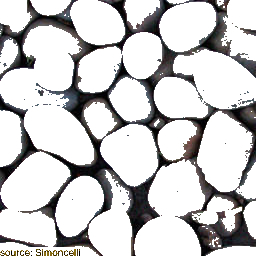
\includegraphics[width=\textwidth]{images/04-experiment01/pebbles/threshold_bg.jpg}
            \caption{Background}
            \vspace*{5mm}
            \label{fig:ex01-pebbles-1000steps-threshold_bg}
        \end{subfigure}
        \hfill
        \begin{subfigure}{0.24\textwidth}
            \centering
            \begin{tikzpicture}
                \draw (0, 0) node[inner sep=0] {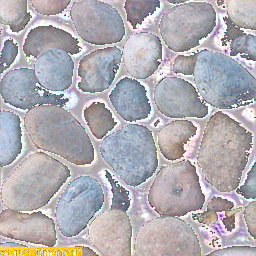
\includegraphics[width=\textwidth]{images/04-experiment01/pebbles/1000/threshold_im.jpg}};
                \fill[black] (-1.55, 1.0) rectangle ++(2.6, 0.6);
                \node [anchor=center] at (-0.25, 1.3) {{\color{white} Ours (Gatys)}};
            \end{tikzpicture}
            \caption{Compensated projection image \(\bm{p}\)}
            \label{fig:ex01-pebbles-1000steps-threshold_im}
        \end{subfigure}
        \hfill
        \begin{subfigure}{0.24\textwidth}
            \centering
            \begin{tikzpicture}
                \draw (0, 0) node[inner sep=0] {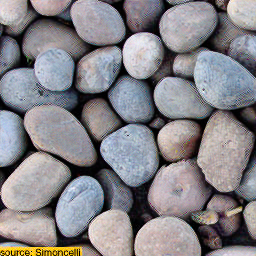
\includegraphics[width=\textwidth]{images/04-experiment01/pebbles/1000/threshold_proj.jpg}};
                \fill[black] (-1.55, 1.0) rectangle ++(2.6, 0.6);
                \node [anchor=center] at (-0.25, 1.3) {{\color{white} Ours (Gatys)}};
            \end{tikzpicture}
            \caption{Final appearance \(r(\bm{p})\)}
            \label{fig:ex01-pebbles-1000steps-threshold_proj}
        \end{subfigure}
    \end{subfigure}
    \caption{Results of experiment 1. We use the simple rendering function (see Section~\ref{section:methods-rendering_function-simple}) and unmodified Gatys texture model (see Section~\ref{section:methods-texture_model}). The background is always a subset of the input texture. Note how feature outlines in background~\ref{fig:ex01-pebbles-1000steps-threshold_bg} completely determine their inner values in the final appearance~\ref{fig:ex01-pebbles-1000steps-threshold_proj}. Also note that the area in~\ref{fig:ex01-pebbles-1000steps-some_proj} where the background matches the input is slightly darker. This is likely caused by~\ref{fig:ex01-pebbles-1000steps-some_im} being initialized by white noise with mean 0.5 and only global brightness enforcement in the texture model. Texture source: \citet{Gatys2015}}
    \label{fig:ex01-pebbles-1000steps}
\end{figure}

\subsection{Results}
\label{section:results-experiments-01-results}

Figure~\ref{fig:ex01-pebbles-1000steps} shows the main result of this experiment. Overall, we have tested five different backgrounds and two different input textures. Complete results can be found in appendix~\ref{chapter:appendix-results} in figs.~\ref{fig:ex01-complete-pebbles-1000steps} and~\ref{fig:ex01-complete-flowers-1000steps}.

Generated compensated projection images \(\bm{p}\) were \(256 \times 256\) large. A single run (one background, one input texture) lasted around 2.5s per 10 optimization steps. All runs were set to perform 1000 steps and reasonable results have started appearing already after around 100 steps (see fig.~\ref{fig:ex01-loss_plot}). The GPU used was Nvidia Tesla K80.

\subsection{Analysis}
\label{section:results-experiments-01-analysis}

\begin{figure}[]
    \centering    
    \begin{subfigure}{\textwidth}
        \centering
        \begin{subfigure}{0.24\textwidth}
            \centering
            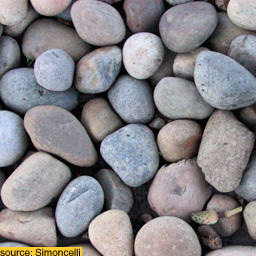
\includegraphics[width=\textwidth]{images/04-experiment01/pebbles/target.jpg}
        \end{subfigure}
        \hfill
        \begin{subfigure}{0.24\textwidth}
            \centering
            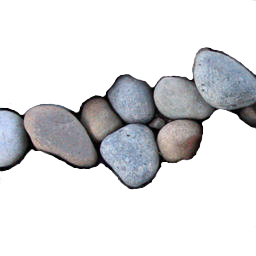
\includegraphics[width=\textwidth]{images/04-experiment01/pebbles/some_bg.jpg}
        \end{subfigure}
        \hfill
        \begin{subfigure}{0.24\textwidth}
            \centering
            \begin{tikzpicture}
                \draw (0, 0) node[inner sep=0] {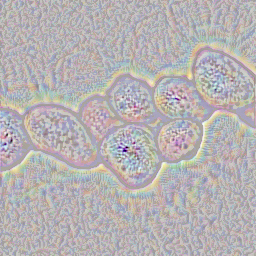
\includegraphics[width=\textwidth]{images/04-experiment01/pebbles/5/some_im.jpg}};
                \fill[black] (-1.55, 1.0) rectangle ++(2.6, 0.6);
                \node [anchor=center] at (-0.25, 1.3) {{\color{white} Ours (Gatys)}};
            \end{tikzpicture}
        \end{subfigure}
        \hfill
        \begin{subfigure}{0.24\textwidth}
            \centering
            \begin{tikzpicture}
                \draw (0, 0) node[inner sep=0] {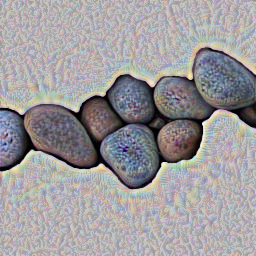
\includegraphics[width=\textwidth]{images/04-experiment01/pebbles/5/some_proj.jpg}};
                \fill[black] (-1.55, 1.0) rectangle ++(2.6, 0.6);
                \node [anchor=center] at (-0.25, 1.3) {{\color{white} Ours (Gatys)}};
            \end{tikzpicture}
        \end{subfigure}
        
        \begin{subfigure}{0.24\textwidth}
            \centering
            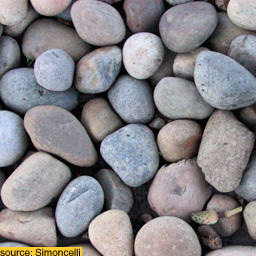
\includegraphics[width=\textwidth]{images/04-experiment01/pebbles/target.jpg}
            \caption*{Desired appearance \(\bm{y}\)}
        \end{subfigure}
        \hfill
        \begin{subfigure}{0.24\textwidth}
            \centering
            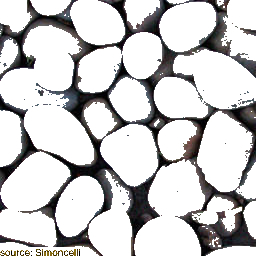
\includegraphics[width=\textwidth]{images/04-experiment01/pebbles/threshold_bg.jpg}
            \caption*{Background}
            \vspace*{5mm}
        \end{subfigure}
        \hfill
        \begin{subfigure}{0.24\textwidth}
            \centering
            \begin{tikzpicture}
                \draw (0, 0) node[inner sep=0] {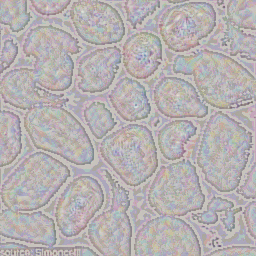
\includegraphics[width=\textwidth]{images/04-experiment01/pebbles/5/threshold_im.jpg}};
                \fill[black] (-1.55, 1.0) rectangle ++(2.6, 0.6);
                \node [anchor=center] at (-0.25, 1.3) {{\color{white} Ours (Gatys)}};
            \end{tikzpicture}
            \caption*{Projection image \(\bm{p}\)}
            \vspace*{5mm}
        \end{subfigure}
        \hfill
        \begin{subfigure}{0.24\textwidth}
            \centering
            \begin{tikzpicture}
                \draw (0, 0) node[inner sep=0] {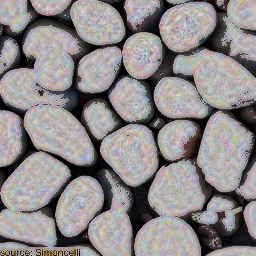
\includegraphics[width=\textwidth]{images/04-experiment01/pebbles/5/threshold_proj.jpg}};
                \fill[black] (-1.55, 1.0) rectangle ++(2.6, 0.6);
                \node [anchor=center] at (-0.25, 1.3) {{\color{white} Ours (Gatys)}};
            \end{tikzpicture}
            \caption*{Appearance \(r(\bm{p})\)}
            \vspace*{5mm}
        \end{subfigure}
    \end{subfigure}
    \caption{A snapshot of experiment 1 after the first five optimization steps which illustrates how the algorithm is initialized and how it converges. Texture source: \citet{Gatys2015}}
    \label{fig:ex01-pebbles-5steps}
\end{figure}

It can be said that our method is indeed capable of controlling the synthesis in a way that yields only such textures that match the background well. The algorithm largely respects the texture features which are already present in the background and continues the texture smoothly around them.

Especially interesting is the second row in figure~\ref{fig:ex01-pebbles-1000steps} where the outlines of all the pebbles are fixed by the background. Our method not only respects those boundaries, but also reproduces the input texture almost perfectly. This is in line with texture theory as discussed in Section~\ref{section:background-texture_synthesis-textures}. The Gatys texture model treats individual pebbles as features that can be shuffled around and their shape can be modified (as in the first row), but once their positions and outlines are fixed, the inner values are largely determined.

In the first row of figure~\ref{fig:ex01-pebbles-1000steps}, we can see that the area where the background matches the input is not fully saturated as expected and as a result, the final appearance is slightly darker in this area. A possible explanation for this is that the algorithm starts from a white noise image with mean \(0.5\) (see figure~\ref{fig:ex01-pebbles-5steps}). Combined with the fact that the loss decreases the fastest at the beginning of the optimization process (see fig.~\ref{fig:ex01-loss_plot}), this likely translates into the algorithm preferring to leave the middle area of the image darker and compensating overall brightness by making the surrounding pebbles brighter, rather than matching the exact appearance of the middle area to that of the input. From the perspective of this experiment, however, this is not a major issue.

\begin{figure}[ht]
    \centering
    \def\svgwidth{0.8\textwidth}
    \input{images/04-experiment01/loss_plot_inkscape.pdf_tex}
    \caption{Loss plot of our projection mapping optimization process suggests that most of the final appearance is determined already after the first few steps. Our loss is defined as the mean square error of the set of statistics of the input (desired appearance) and the final camera image (see fig.~\ref{fig:methods_pipeline} for more details).}
    \label{fig:ex01-loss_plot}
\end{figure}

\section{Evaluating various texture models}
\label{section:results-experiments-02}

In the first experiment, we have shown that our method is able to converge to the desired result in certain toy examples. We now focus on how the texture model influences the performance of our method. We also compare against a conventional pixel-based algorithm in a variety of more challenging scenes.

\textbf{Goal.} We want to compare the performance of three different methods:

\begin{itemize}
    \item Conventional pixel-based projection mapping (baseline)
    \item Ours with the original Gatys texture model
    \item Ours with the improved texture model (we use the Pyramid + Shift variant from Section~\ref{section:methods-texture_model-improvements} because it performs best when synthesizing textures)
\end{itemize}

\textbf{Setup.} We keep using the simple rendering function (see Section~\ref{section:methods-rendering_function-simple}) because what makes a scene challenging is the fact that the projector is not bright enough to achieve a particular appearance. The simple rendering function is sufficient to reproduce these conditions. We set the constant \(c\) (see eq.~\ref{eq:rendering_function-simple}) to adjust the difficulty of each scene. As for the texture models, we use both the original Gatys texture model (see Section~\ref{section:methods-texture_model}) and its improved variant (in particular, we use the Pyramid + Shift variant as described in~\ref{section:methods-texture_model-improvements}). We obtain the pixel-based baseline by removing the statistics-based loss from our pipeline (see Section~\ref{section:methods-pipeline_overview}) and replacing it with a per-pixel L2 difference between the input texture and the camera image. This approach yields an algorithm which solves eq.~\ref{eq:projection_mapping-per_pixel} and is thus the optimal pixel-based projection mapping algorithm. The inputs to this experiment are pairs of scene (represented by a background image) and texture image \(\bm{y}\) that we wish to map onto the scene.

\subsection{Results}
\label{section:results-experiments-02-results}

\begin{figure}[]
    \centering    
    \begin{subfigure}{\textwidth}
        \centering
        \begin{subfigure}{0.2\textwidth}
            \centering
            \vspace*{5mm}
            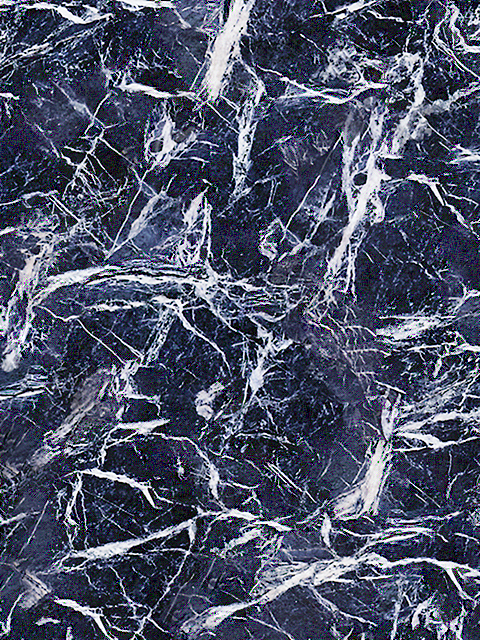
\includegraphics[width=\textwidth]{images/04-experiment02/human/marble/target.jpg}
            \caption*{Desired appearance \(\bm{y}\)}
        \end{subfigure}
        \hfill
        \begin{subfigure}{0.78\textwidth}
            \centering
            \begin{subfigure}{0.32\textwidth}
                \centering
                \begin{tikzpicture}
                    \draw (0, 0) node[inner sep=0] {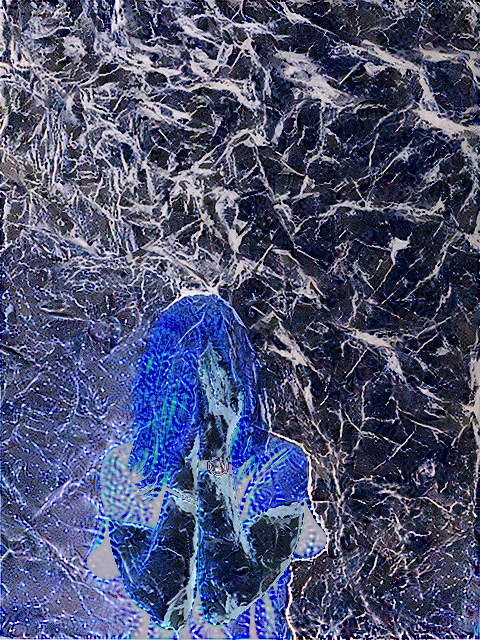
\includegraphics[width=\textwidth]{images/04-experiment02/human/marble/gatys_im.jpg}};
                    \fill[black] (-1.0, 1.6) rectangle ++(2.6, 0.6);
                    \node [anchor=center] at (0.3, 1.9) {{\color{white} Ours (Gatys)}};
                \end{tikzpicture}
            \end{subfigure}
            \hfill
            \begin{subfigure}{0.32\textwidth}
                \centering
                \begin{tikzpicture}
                    \draw (0, 0) node[inner sep=0] {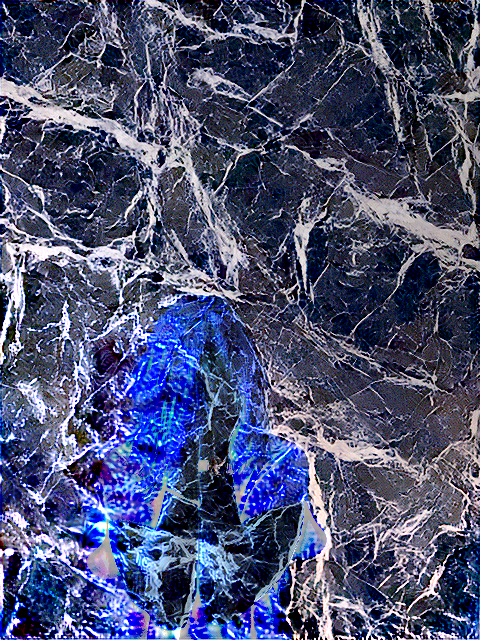
\includegraphics[width=\textwidth]{images/04-experiment02/human/marble/improved_im.jpg}};
                    \fill[black] (-1.5, 1.6) rectangle ++(3.1, 0.6);
                    \node [anchor=center] at (0.05, 1.88) {{\color{white} \small{Ours (Improved)}}};
                \end{tikzpicture}
            \end{subfigure}
            \hfill
            \begin{subfigure}{0.32\textwidth}
                \centering
                \begin{tikzpicture}
                    \draw (0, 0) node[inner sep=0] {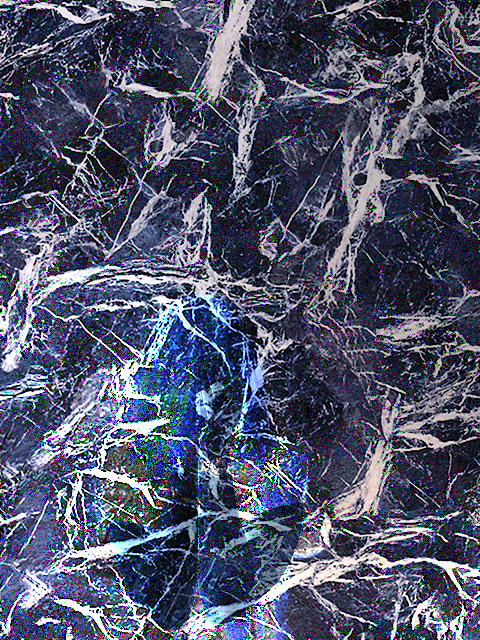
\includegraphics[width=\textwidth]{images/04-experiment02/human/marble/pixel_im.jpg}};
                    \fill[black] (-1.0, 1.6) rectangle ++(2.6, 0.6);
                    \node [anchor=center] at (0.3, 1.9) {{\color{white} Baseline}};
                \end{tikzpicture}
            \end{subfigure}
            \caption*{Compensated projection image \(\bm{p}\)}
        \end{subfigure}
        
        \begin{subfigure}{0.2\textwidth}
            \centering
            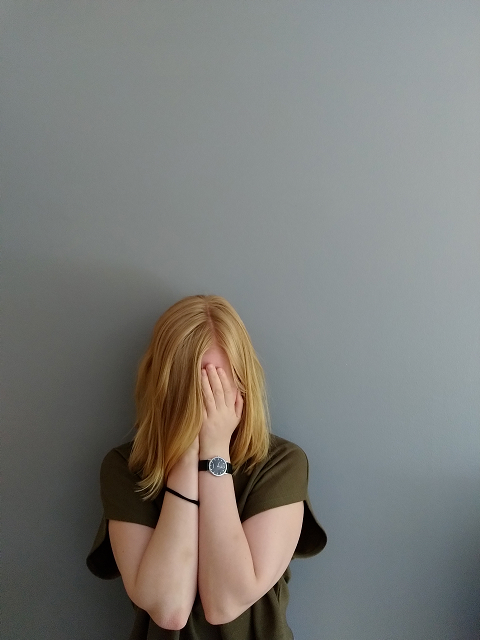
\includegraphics[width=\textwidth]{images/04-experiment02/human/bg.jpg}
            \caption*{Background}
        \end{subfigure}
        \hfill
        \begin{subfigure}{0.78\textwidth}
            \begin{subfigure}{0.32\textwidth}
                \centering
                \begin{tikzpicture}
                    \draw (0, 0) node[inner sep=0] {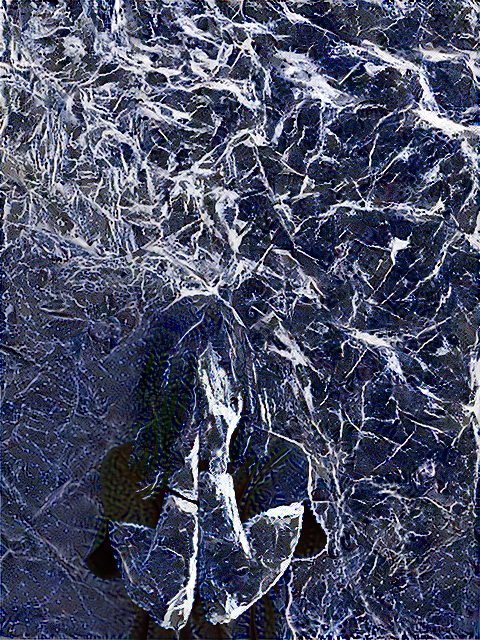
\includegraphics[width=\textwidth]{images/04-experiment02/human/marble/gatys_proj.jpg}};
                    \fill[black] (-1.0, 1.6) rectangle ++(2.6, 0.6);
                    \node [anchor=center] at (0.3, 1.9) {{\color{white} Ours (Gatys)}};
                    \draw[line width=0.4mm, green] (-0.75, -0.85) rectangle ++(0.93, 1.0);
                    \draw[line width=0.4mm, orange] (-1.12, -2.2) rectangle ++(1.75, 1.0);
                    \draw[line width=0.4mm, red] (-1.65, -2.2) rectangle ++(0.48, 1.0);
                \end{tikzpicture}
            \end{subfigure}
            \hfill
            \begin{subfigure}{0.32\textwidth}
                \centering
                \begin{tikzpicture}
                    \draw (0, 0) node[inner sep=0] {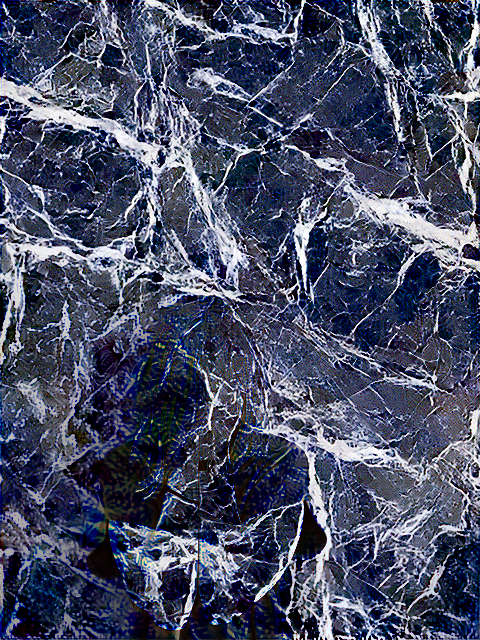
\includegraphics[width=\textwidth]{images/04-experiment02/human/marble/improved_proj.jpg}};
                    \fill[black] (-1.5, 1.6) rectangle ++(3.1, 0.6);
                    \node [anchor=center] at (0.05, 1.88) {{\color{white} \small{Ours (Improved)}}};
                    \draw[line width=0.4mm, green] (-0.75, -0.85) rectangle ++(0.93, 1.0);
                    \draw[line width=0.4mm, orange] (-1.12, -2.2) rectangle ++(1.75, 1.0);
                    \draw[line width=0.4mm, red] (-1.65, -2.2) rectangle ++(0.48, 1.0);
                \end{tikzpicture}
            \end{subfigure}
            \hfill
            \begin{subfigure}{0.32\textwidth}
                \centering
                \begin{tikzpicture}
                    \draw (0, 0) node[inner sep=0] {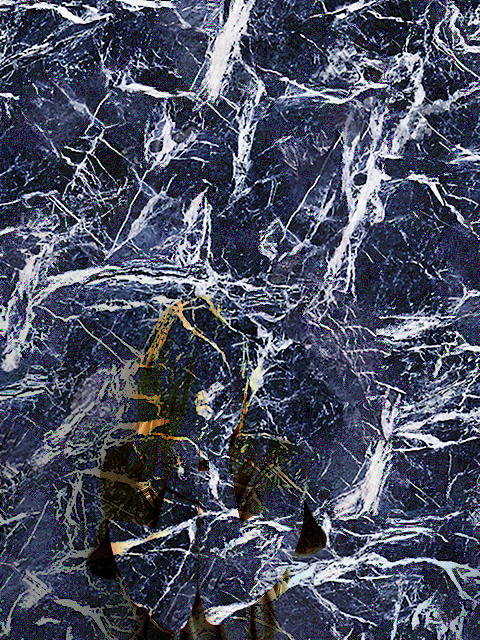
\includegraphics[width=\textwidth]{images/04-experiment02/human/marble/pixel_proj.jpg}};
                    \fill[black] (-1.0, 1.6) rectangle ++(2.6, 0.6);
                    \node [anchor=center] at (0.3, 1.9) {{\color{white} Baseline}};
                    \draw[line width=0.4mm, green] (-0.75, -0.85) rectangle ++(0.93, 1.0);
                    \draw[line width=0.4mm, orange] (-1.12, -2.2) rectangle ++(1.75, 1.0);
                    \draw[line width=0.4mm, red] (-1.65, -2.2) rectangle ++(0.48, 1.0);
                \end{tikzpicture}
            \end{subfigure}
            \caption*{Final appearance \(r(\bm{p})\)}
        \end{subfigure}

        \hfill
        \begin{subfigure}{0.78\textwidth}
            \centering
            \begin{subfigure}{0.32\textwidth}
                \centering
                \begin{subfigure}{0.32\textwidth}
                    \centering
                    \begin{tikzpicture}
                        \draw (0, 0) node[inner sep=0] {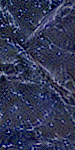
\includegraphics[width=\textwidth]{images/04-experiment02/human/marble/gatys_proj_crop_red.jpg}};
                        \draw[line width=0.4mm, red] (-0.55, -1.08) rectangle ++(1.1, 2.16);
                    \end{tikzpicture}
                \end{subfigure}
                \hfill
                \begin{subfigure}{0.6\textwidth}
                    \centering
                    \begin{tikzpicture}
                        \draw (0, 0) node[inner sep=0] {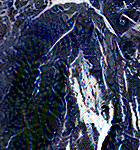
\includegraphics[width=\textwidth]{images/04-experiment02/human/marble/gatys_proj_crop_green.jpg}};
                        \draw[line width=0.4mm, green] (-1.0, -1.08) rectangle ++(2.02, 2.16);
                    \end{tikzpicture}
                \end{subfigure}
    
                \begin{subfigure}{\textwidth}
                    \centering
                    \begin{tikzpicture}
                        \draw (0, 0) node[inner sep=0] {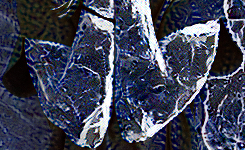
\includegraphics[width=\textwidth]{images/04-experiment02/human/marble/gatys_proj_crop_yellow.jpg}};
                        \draw[line width=0.4mm, orange] (-1.7, -1.06) rectangle ++(3.4, 2.12);
                    \end{tikzpicture}
                \end{subfigure}
            \end{subfigure}
            \begin{subfigure}{0.32\textwidth}
                \centering
                \begin{subfigure}{0.32\textwidth}
                    \centering
                    \begin{tikzpicture}
                        \draw (0, 0) node[inner sep=0] {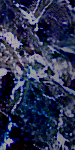
\includegraphics[width=\textwidth]{images/04-experiment02/human/marble/improved_proj_crop_red.jpeg}};
                        \draw[line width=0.4mm, red] (-0.55, -1.08) rectangle ++(1.1, 2.16);
                    \end{tikzpicture}
                \end{subfigure}
                \hfill
                \begin{subfigure}{0.6\textwidth}
                    \centering
                    \begin{tikzpicture}
                        \draw (0, 0) node[inner sep=0] {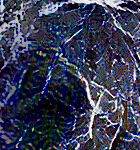
\includegraphics[width=\textwidth]{images/04-experiment02/human/marble/improved_proj_crop_green.jpeg}};
                        \draw[line width=0.4mm, green] (-1.0, -1.08) rectangle ++(2.02, 2.16);
                    \end{tikzpicture}
                \end{subfigure}
    
                \begin{subfigure}{\textwidth}
                    \centering
                    \begin{tikzpicture}
                        \draw (0, 0) node[inner sep=0] {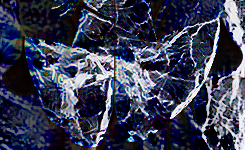
\includegraphics[width=\textwidth]{images/04-experiment02/human/marble/improved_proj_crop_yellow.jpeg}};
                        \draw[line width=0.4mm, orange] (-1.7, -1.06) rectangle ++(3.4, 2.12);
                    \end{tikzpicture}
                \end{subfigure}
            \end{subfigure}
            \begin{subfigure}{0.32\textwidth}
                \centering
                \begin{subfigure}{0.32\textwidth}
                    \centering
                    \begin{tikzpicture}
                        \draw (0, 0) node[inner sep=0] {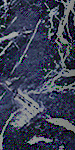
\includegraphics[width=\textwidth]{images/04-experiment02/human/marble/pixel_proj_crop_red.jpeg}};
                        \draw[line width=0.4mm, red] (-0.55, -1.08) rectangle ++(1.1, 2.16);
                    \end{tikzpicture}
                \end{subfigure}
                \hfill
                \begin{subfigure}{0.6\textwidth}
                    \centering
                    \begin{tikzpicture}
                        \draw (0, 0) node[inner sep=0] {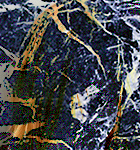
\includegraphics[width=\textwidth]{images/04-experiment02/human/marble/pixel_proj_crop_green.jpeg}};
                        \draw[line width=0.4mm, green] (-1.0, -1.08) rectangle ++(2.02, 2.16);
                    \end{tikzpicture}
                \end{subfigure}
    
                \begin{subfigure}{\textwidth}
                    \centering
                    \begin{tikzpicture}
                        \draw (0, 0) node[inner sep=0] {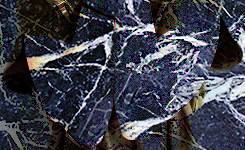
\includegraphics[width=\textwidth]{images/04-experiment02/human/marble/pixel_proj_crop_yellow.jpeg}};
                        \draw[line width=0.4mm, orange] (-1.7, -1.06) rectangle ++(3.4, 2.12);
                    \end{tikzpicture}
                \end{subfigure}
            \end{subfigure}
            \caption*{Details}
        \end{subfigure}
    \end{subfigure}
    \caption{Results of experiment 2. We use the simple rendering function (see Section~\ref{section:methods-rendering_function-simple}) and compare our method with the original Gatys texture model (see Section~\ref{section:methods-texture_model}) against our method with the improved texture model (specifically, the Pyramid + Shift variant from Section~\ref{section:methods-texture_model-improvements}) and a conventional pixel-based projection mapping method. Brightness \(c\) is set to \(5\) to adjust the difficulty of the scene. Note in the details how our method with the improved model is better than Gatys at matching the large features of the input (e.g.~the outline of the woman is not visible and the size of the marble grain stays roughly the same). It is also better than the pixel-based method at matching the colours (e.g.~the blond hair is not visible in the final appearance). Texture source: \citet{Pixar128}}
    \label{fig:ex02-human-marble}
\end{figure}

Figure~\ref{fig:ex02-human-marble} shows the main result of this experiment. Overall, we have tested four different backgrounds and five different input textures. The brightness constant \(c\) was set to \(5\) in all cases, meaning that the texture was first multiplied by \(5\) before being projected (see eq.~\ref{eq:rendering_function-simple}). Complete results of those runs can be found in appendix~\ref{chapter:appendix-results} in figs.~\ref{fig:ex02-complete-human-marble_wood}, \ref{fig:ex02-complete-human-flowers_flowers2}, \ref{fig:ex02-complete-human-pebbles}, \ref{fig:ex02-complete-carpet-marble_wood_pebbles}, \ref{fig:ex02-complete-carpet-flowers_flowers2}, \ref{fig:ex02-complete-sofa-marble_wood_pebbles}, \ref{fig:ex02-complete-sofa-flowers_flowers2}, \ref{fig:ex02-complete-photo-marble_wood_pebbles} and \ref{fig:ex02-complete-photo-flowers_flowers2}.

Generated compensated projection images \(\bm{p}\) were \(640 \times 480\) large. A single run (one background, one input texture) lasted around 11s per 10 optimization steps. All runs were set to perform 1000 steps and reasonable results have started appearing already after around 100 steps (see fig.~\ref{fig:ex01-loss_plot}). The GPU used was Nvidia Tesla K80.

\subsection{Analysis}
\label{section:results-experiments-02-analysis}

\begin{figure}[]
    \centering    
    \begin{subfigure}{\textwidth}
        \centering
        \begin{subfigure}{0.19\textwidth}
            \centering
            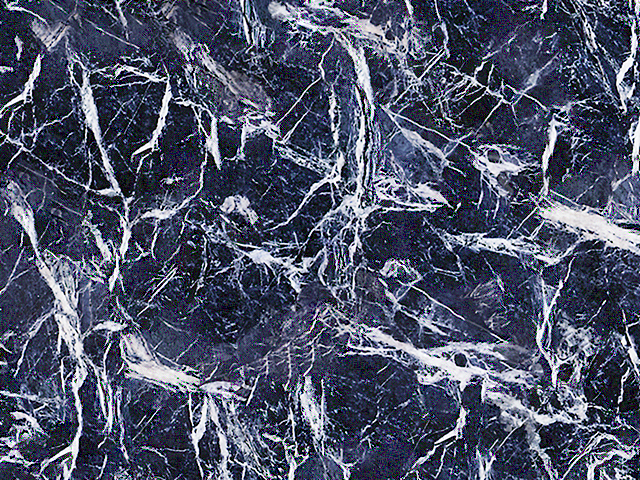
\includegraphics[width=\textwidth]{images/04-experiment02/isolating_issues/target.jpg}
        \end{subfigure}
        \hfill
        \begin{subfigure}{0.19\textwidth}
            \centering
            
\includegraphics[width=\textwidth]{images/04-experiment02/isolating_issues/255_bg.jpg}
        \end{subfigure}
        \hfill
        \begin{subfigure}{0.6\textwidth}
            \centering
            \begin{subfigure}{0.32\textwidth}
                \centering
                \begin{tikzpicture}
                    \draw (0, 0) node[inner sep=0] {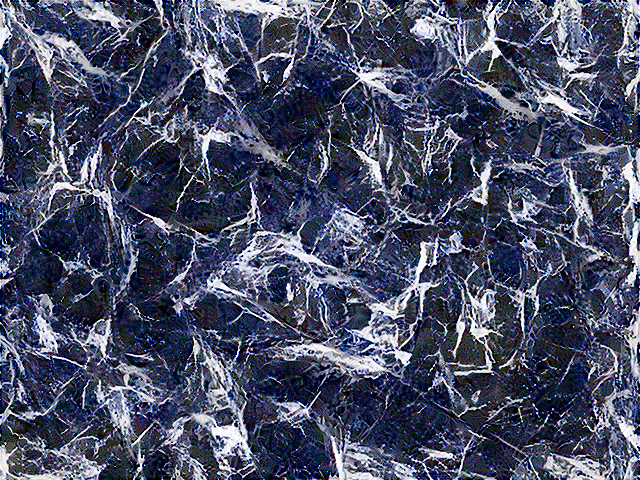
\includegraphics[width=\textwidth]{images/04-experiment02/isolating_issues/255_gatys.jpg}};
                    \fill[black] (-1.2, 0.45) rectangle ++(2.4, 0.5);
                    \node [anchor=center] at (0.0, 0.69) {{\footnotesize{\color{white} Ours (Gatys)}}};
                \end{tikzpicture}
            \end{subfigure}
            \hfill
            \begin{subfigure}{0.32\textwidth}
                \centering
                \begin{tikzpicture}
                    \draw (0, 0) node[inner sep=0] {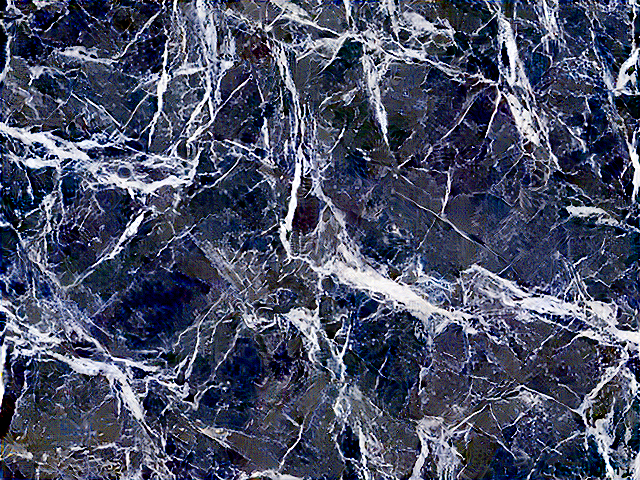
\includegraphics[width=\textwidth]{images/04-experiment02/isolating_issues/255_improved.jpg}};
                    \fill[black] (-1.25, 0.45) rectangle ++(2.5, 0.5);
                    \node [anchor=center] at (0.0, 0.69) {{\scriptsize{\color{white} Ours (Improved)}}};
                \end{tikzpicture}
            \end{subfigure}
            \hfill
            \begin{subfigure}{0.32\textwidth}
                \centering
                \begin{tikzpicture}
                    \draw (0, 0) node[inner sep=0] {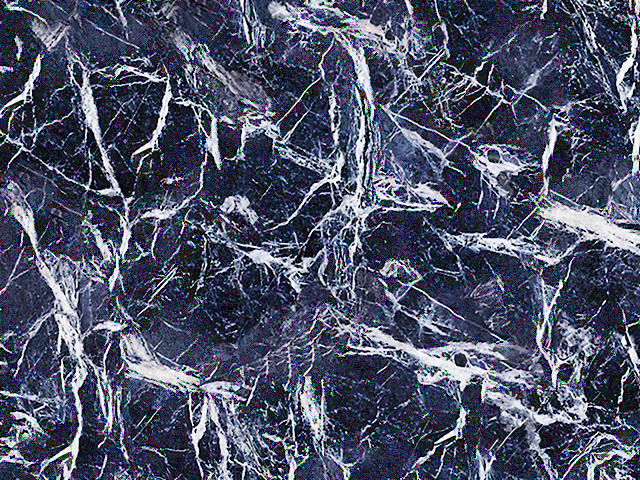
\includegraphics[width=\textwidth]{images/04-experiment02/isolating_issues/255_pixel.jpg}};
                    \fill[black] (-1.2, 0.45) rectangle ++(2.4, 0.5);
                    \node [anchor=center] at (0.0, 0.69) {{\footnotesize{\color{white} Baseline}}};
                \end{tikzpicture}
            \end{subfigure}
        \end{subfigure}
        
        \begin{subfigure}{0.19\textwidth}
            \centering
            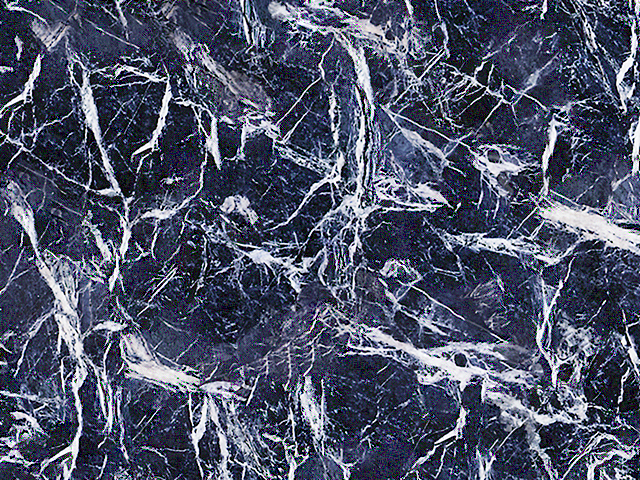
\includegraphics[width=\textwidth]{images/04-experiment02/isolating_issues/target.jpg}
        \end{subfigure}
        \hfill
        \begin{subfigure}{0.19\textwidth}
            \centering
            
\includegraphics[width=\textwidth]{images/04-experiment02/isolating_issues/210_bg.jpg}
        \end{subfigure}
        \hfill
        \begin{subfigure}{0.6\textwidth}
            \centering
            \begin{subfigure}{0.32\textwidth}
                \centering
                \begin{tikzpicture}
                    \draw (0, 0) node[inner sep=0] {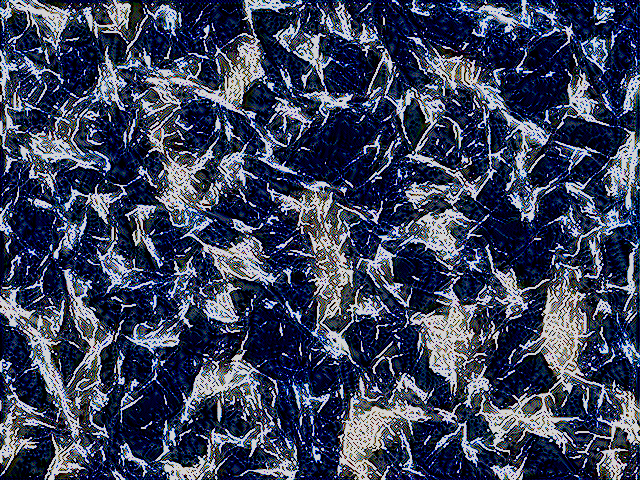
\includegraphics[width=\textwidth]{images/04-experiment02/isolating_issues/210_gatys.jpg}};
                    \fill[black] (-1.2, 0.45) rectangle ++(2.4, 0.5);
                    \node [anchor=center] at (0.0, 0.69) {{\footnotesize{\color{white} Ours (Gatys)}}};
                \end{tikzpicture}
            \end{subfigure}
            \hfill
            \begin{subfigure}{0.32\textwidth}
                \centering
                \begin{tikzpicture}
                    \draw (0, 0) node[inner sep=0] {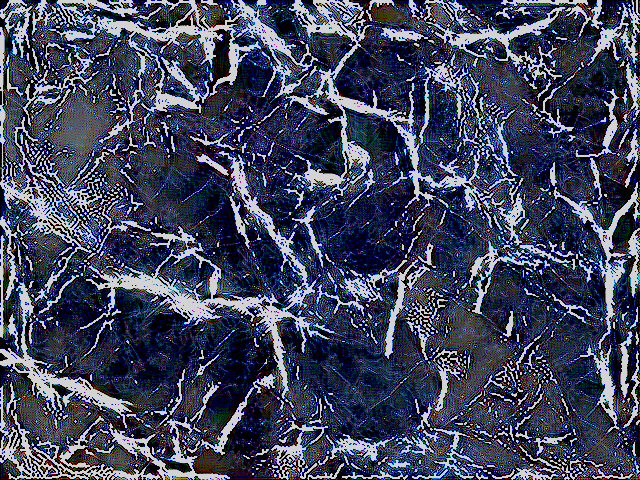
\includegraphics[width=\textwidth]{images/04-experiment02/isolating_issues/210_improved.jpg}};
                    \fill[black] (-1.25, 0.45) rectangle ++(2.5, 0.5);
                    \node [anchor=center] at (0.0, 0.69) {{\scriptsize{\color{white} Ours (Improved)}}};
                \end{tikzpicture}
            \end{subfigure}
            \hfill
            \begin{subfigure}{0.32\textwidth}
                \centering
                \begin{tikzpicture}
                    \draw (0, 0) node[inner sep=0] {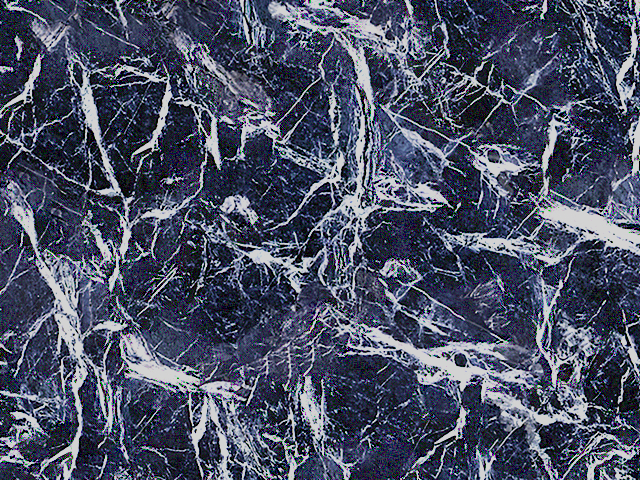
\includegraphics[width=\textwidth]{images/04-experiment02/isolating_issues/210_pixel.jpg}};
                    \fill[black] (-1.2, 0.45) rectangle ++(2.4, 0.5);
                    \node [anchor=center] at (0.0, 0.69) {{\footnotesize{\color{white} Baseline}}};
                \end{tikzpicture}
            \end{subfigure}
        \end{subfigure}

        \begin{subfigure}{0.19\textwidth}
            \centering
            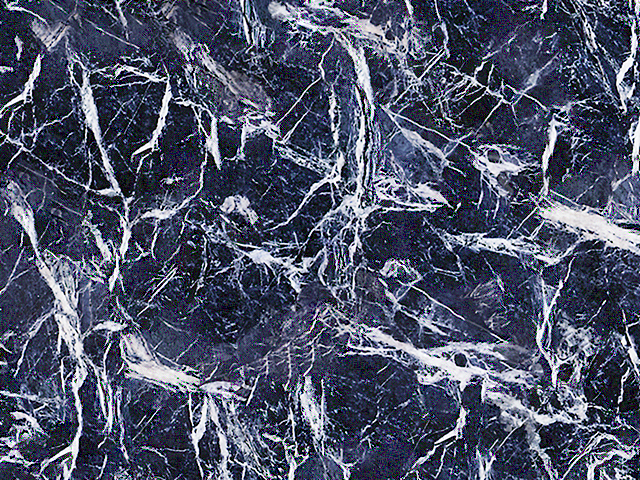
\includegraphics[width=\textwidth]{images/04-experiment02/isolating_issues/target.jpg}
            \caption*{Desired appearance \(\bm{y}\)}
        \end{subfigure}
        \hfill
        \begin{subfigure}{0.19\textwidth}
            \centering
            
\includegraphics[width=\textwidth]{images/04-experiment02/isolating_issues/190_bg.jpg}
            \caption*{Background}
            \vspace*{5mm}
        \end{subfigure}
        \hfill
        \begin{subfigure}{0.6\textwidth}
            \centering
            \begin{subfigure}{0.32\textwidth}
                \centering
                \begin{tikzpicture}
                    \draw (0, 0) node[inner sep=0] {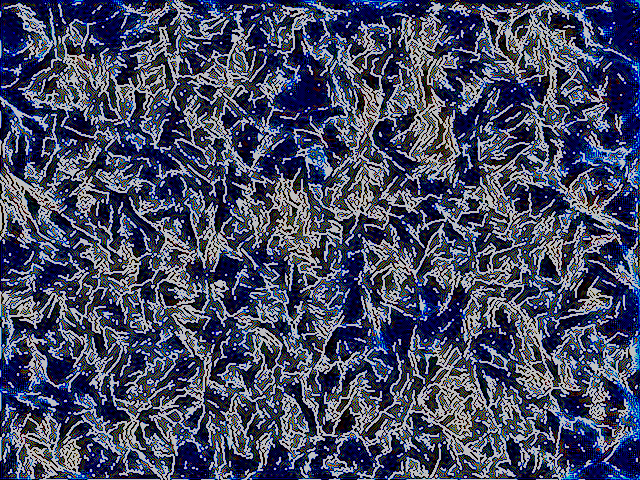
\includegraphics[width=\textwidth]{images/04-experiment02/isolating_issues/190_gatys.jpg}};
                    \fill[black] (-1.2, 0.45) rectangle ++(2.4, 0.5);
                    \node [anchor=center] at (0.0, 0.69) {{\footnotesize{\color{white} Ours (Gatys)}}};
                \end{tikzpicture}
            \end{subfigure}
            \hfill
            \begin{subfigure}{0.32\textwidth}
                \centering
                \begin{tikzpicture}
                    \draw (0, 0) node[inner sep=0] {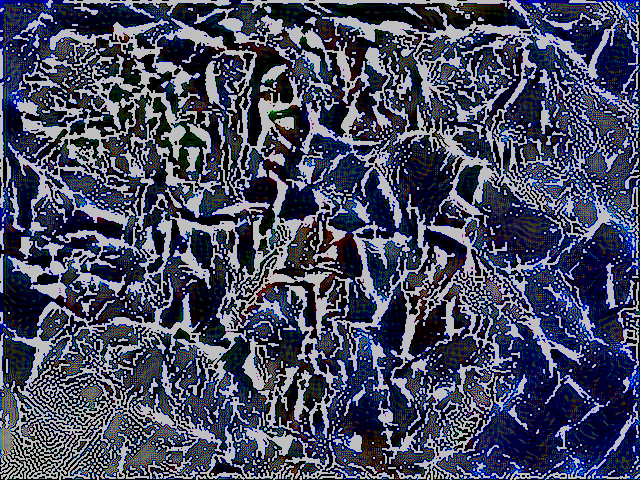
\includegraphics[width=\textwidth]{images/04-experiment02/isolating_issues/190_improved.jpg}};
                    \fill[black] (-1.25, 0.45) rectangle ++(2.5, 0.5);
                    \node [anchor=center] at (0.0, 0.69) {{\scriptsize{\color{white} Ours (Improved)}}};
                \end{tikzpicture}
            \end{subfigure}
            \hfill
            \begin{subfigure}{0.32\textwidth}
                \centering
                \begin{tikzpicture}
                    \draw (0, 0) node[inner sep=0] {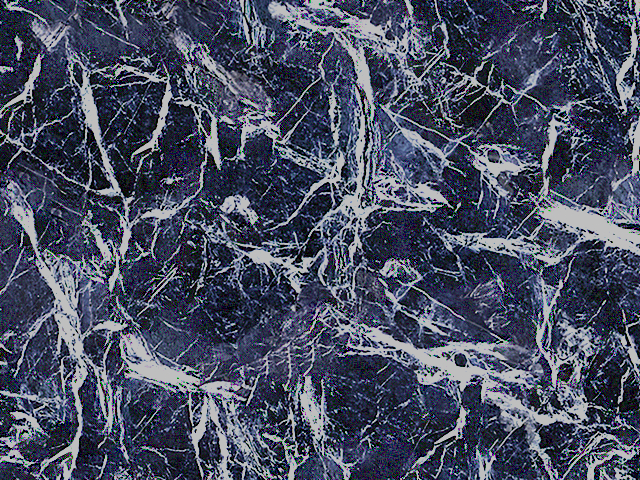
\includegraphics[width=\textwidth]{images/04-experiment02/isolating_issues/190_pixel.jpg}};
                    \fill[black] (-1.2, 0.45) rectangle ++(2.4, 0.5);
                    \node [anchor=center] at (0.0, 0.69) {{\footnotesize{\color{white} Baseline}}};
                \end{tikzpicture}
            \end{subfigure}
            \caption*{Final appearance \(r(\bm{p})\)}
            \vspace*{5mm}
        \end{subfigure}
        
    \end{subfigure}
    \caption{A study of convergence of our method when the overall intensity of the input cannot be recovered by the projector due to dark background. \(c = 1\) in this case. The last three images in each row show the final appearance \(r(\bm{p})\) for each compared method. The upper row corresponds to texture synthesis since the background is pure white. Background in the middle row has grey level of 210 out of 255, while background in the lower row has grey level of 190 out of 255. Note how the ability to recover large texture features rapidly degrades with darkening background. Also note how the improved texture model performs better than the Gatys model. The pixel-based baseline handles these extreme situations better since it only tries to match the intensity of each pixel while texture features are simply equal to the input. Texture source: \citet{Pixar128}}
    \label{fig:ex02-issues}
\end{figure}

When comparing the three methods -- ours with the Gatys texture model, ours with the improved texture model and the pixel-based baseline -- it is useful to think in terms of micro- and macro-textures (as introduced in Section~\ref{section:background-texture_synthesis-statistics_based}). For example, in a pebble texture like the one in figure~\ref{section:results-experiments-01-results}, the pebbles themselves form a macro-texture while their surface is a micro-texture.

Starting with our method with the Gatys texture model in fig.~\ref{fig:ex02-human-marble}, we can see that it reproduces micro-texture very well. The resulting appearance contains mostly colours from the input texture and colours of the background, for example the blond hair, are hidden, unlike in the pixel-based baseline. On the other hand, macro-texture is recovered rather poorly as the outline of the woman is visible quite clearly. The appearance of large texture features seems to further deteriorate in areas where the background is darker (and thus less reflective), especially in the lower left corner.

In a sense, this is an extreme case. The background in the lower left corner is clearly too dark for the projector to compensate it and at the same time it is too large for texture synthesis to place a dark part of the texture over it. On the other hand, the pixel-based baseline clearly looks better in this area. Where synthesis cannot recover the colour, it does not recover the macro features either, whereas the pixel-based method has the advantage of only needing to match colours and overall, darker appearance with the correct macro features looks better. We have conducted a separate experiment to evaluate the macro feature recovery of the two different texture models in situations where colour cannot be matched. The result is shown in figure~\ref{fig:ex02-issues} and suggests that there are indeed issues with convergence when the overall intensity cannot be achieved. It also shows, however, that the improved texture model performs slightly better in this case.

The improved texture model is clearly better than the original Gatys model in the main result (fig.~\ref{fig:ex02-human-marble}) as well. It recovers micro-texture better than the pixel-based method and its macro-texture is better than that of the Gatys texture model. Overall, we believe that our method provides a more visually pleasing and balanced result than both other methods. At the same time, it seems that potential future improvements in the performance of texture synthesis will also translate into improved statistics-based projection mapping.

\section{Evaluating a general rendering function}
\label{section:results-experiments-03}

The second experiment has shown that statistics-based projection mapping can be a viable alternative to traditional pixel-based approaches, outperforming them in certain situations. However, so far we have only tested our method in the simplified scenario of projecting onto a flat diffuse surface. The last experiment represents a step towards real world deployment of our method and involves projecting onto arbitrary 3D scenes.

\textbf{Goal.} We want to see how the behaviour of our method from previous experiments translates into a more general case of projecting onto arbitrary 3D scenes.

\textbf{Setup.} We now use the general rendering function (see Section~\ref{section:methods-rendering_function-general}) in our pipeline. We also use the improved texture model and the pixel-based baseline for comparison. The inputs to this experiment are pairs of scene (represented by a pre-captured light transport matrix) and texture image \(\bm{y}\) that we wish to map onto the scene. To keep the light transport matrix size manageable, we use projector and camera image size of \(160 \times 160\).

\subsection{Results}
\label{section:results-experiments-03-results}

\begin{figure}[]
    \centering    
    \begin{subfigure}{\textwidth}
        \centering
        \begin{subfigure}{0.5\textwidth}
            \centering
            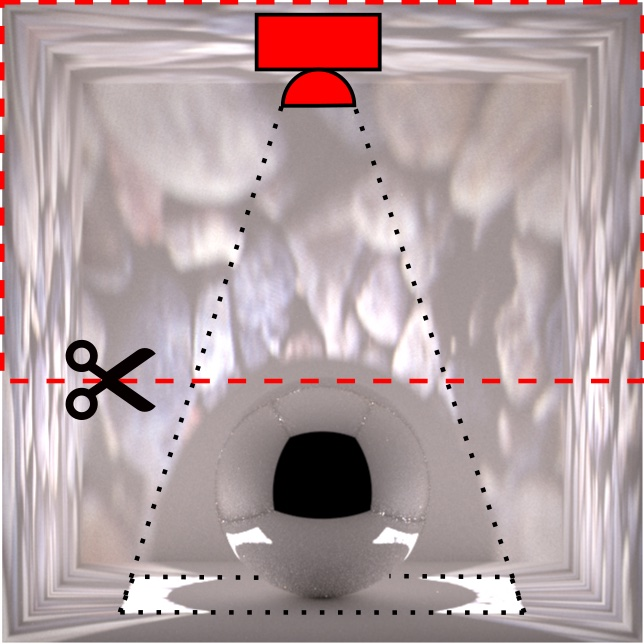
\includegraphics[width=\textwidth]{images/04-experiment03/ball_dof/scene_highlighted.jpg}
            \caption*{Scene}
        \end{subfigure}

        \begin{subfigure}{0.19\textwidth}
            \centering
            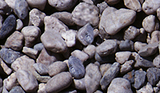
\includegraphics[width=\textwidth]{images/04-experiment03/ball_pebble_target.jpg}
        \end{subfigure}
        \hfill
        \begin{subfigure}{0.19\textwidth}
            \centering
            \begin{tikzpicture}
                \draw (0, 0) node[inner sep=0] {\includegraphics[width=\textwidth]{images/04-experiment03/ball_dof/pebbles/stats_im.jpg}};
                \fill[black] (-1.2, -1.2) rectangle ++(2.4, 0.5);
                \node [anchor=center] at (0.0, -0.95) {{\color{white} \scriptsize{Ours (Improved)}}};
            \end{tikzpicture}
        \end{subfigure}
        \hfill
        \begin{subfigure}{0.19\textwidth}
            \centering
            \begin{tikzpicture}
                \draw (0, 0) node[inner sep=0] {\includegraphics[width=\textwidth]{images/04-experiment03/ball_dof/pebbles/stats_proj_highlighted.jpg}};
                \fill[black] (-1.2, -1.2) rectangle ++(2.4, 0.5);
                \node [anchor=center] at (0.0, -0.95) {{\color{white} \scriptsize{Ours (Improved)}}};
            \end{tikzpicture}
        \end{subfigure}
        \hfill
        \begin{subfigure}{0.19\textwidth}
            \centering
            \begin{tikzpicture}
                \draw (0, 0) node[inner sep=0] {\includegraphics[width=\textwidth]{images/04-experiment03/ball_dof/pebbles/pixel_im.jpg}};
                \fill[black] (-1.2, -1.2) rectangle ++(1.8, 0.5);
                \node [anchor=center] at (-0.3, -0.95) {{\color{white} \small{Baseline}}};
            \end{tikzpicture}
        \end{subfigure}
        \hfill
        \begin{subfigure}{0.19\textwidth}
            \centering
            \begin{tikzpicture}
                \draw (0, 0) node[inner sep=0] {\includegraphics[width=\textwidth]{images/04-experiment03/ball_dof/pebbles/pixel_proj_highlighted.jpg}};
                \fill[black] (-1.2, -1.2) rectangle ++(1.8, 0.5);
                \node [anchor=center] at (-0.3, -0.95) {{\color{white} \small{Baseline}}};
            \end{tikzpicture}
        \end{subfigure}
        
        \begin{subfigure}{0.19\textwidth}
            \centering
            \includegraphics[width=\textwidth]{images/04-experiment03/ball_marble_target.jpg}
            \vspace*{1mm}
            \caption*{Desired appearance \(\bm{y}\)}
        \end{subfigure}
        \hfill
        \begin{subfigure}{0.19\textwidth}
            \centering
            \begin{tikzpicture}
                \draw (0, 0) node[inner sep=0] {\includegraphics[width=\textwidth]{images/04-experiment03/ball_dof/marble/stats_im.jpg}};
                \fill[black] (-1.2, -1.2) rectangle ++(2.4, 0.5);
                \node [anchor=center] at (0.0, -0.95) {{\color{white} \scriptsize{Ours (Improved)}}};
            \end{tikzpicture}
            \caption*{Compensated projection image \(\bm{p}\)}
        \end{subfigure}
        \hfill
        \begin{subfigure}{0.19\textwidth}
            \centering
            \begin{tikzpicture}
                \draw (0, 0) node[inner sep=0] {\includegraphics[width=\textwidth]{images/04-experiment03/ball_dof/marble/stats_proj_highlighted.jpg}};
                \fill[black] (-1.2, -1.2) rectangle ++(2.4, 0.5);
                \node [anchor=center] at (0.0, -0.95) {{\color{white} \scriptsize{Ours (Improved)}}};
            \end{tikzpicture}
            \caption*{Final appearance \(r(\bm{p})\)}
        \end{subfigure}
        \hfill
        \begin{subfigure}{0.19\textwidth}
            \centering
            \begin{tikzpicture}
                \draw (0, 0) node[inner sep=0] {\includegraphics[width=\textwidth]{images/04-experiment03/ball_dof/marble/pixel_im.jpg}};
                \fill[black] (-1.2, -1.2) rectangle ++(1.8, 0.5);
                \node [anchor=center] at (-0.3, -0.95) {{\color{white} \small{Baseline}}};
            \end{tikzpicture}
            \caption*{Compensated projection image \(\bm{p}\)}
        \end{subfigure}
        \hfill
        \begin{subfigure}{0.19\textwidth}
            \centering
            \begin{tikzpicture}
                \draw (0, 0) node[inner sep=0] {\includegraphics[width=\textwidth]{images/04-experiment03/ball_dof/marble/pixel_proj_highlighted.jpg}};
                \fill[black] (-1.2, -1.2) rectangle ++(1.8, 0.5);
                \node [anchor=center] at (-0.3, -0.95) {{\color{white} \small{Baseline}}};
            \end{tikzpicture}
            \caption*{Final appearance \(r(\bm{p})\)}
        \end{subfigure}
    \end{subfigure}
    \caption{Results of experiment 3. We use the general rendering function (see section ~\ref{section:methods-rendering_function-general}) and compare our method with the improved texture model (see Section~\ref{section:methods-texture_model-improvements}) against a pixel-based baseline. \(c = 5\). The scene contains a mirror ball which is being projected onto from the ceiling as suggested in the scene image. The projector has depth of field enabled and the camera image \(r(\bm{p})\) is cropped before computing the loss and thus only the dashed red rectangles are matched against the desired appearance \(\bm{y}\). Overall, our pipeline handles this complex light transport well. Note how the box is missing one wall (the black patch inside the mirror ball) which causes the optimization to leave the corresponding part of the compensation image \(\bm{p}\) untouched. Texture source: \citet{Pixar128}}
    \label{fig:ex03-ball_dof}
\end{figure}

\begin{figure}[]
    \centering    
    \begin{subfigure}{\textwidth}
        \centering
        \begin{subfigure}{0.5\textwidth}
            \centering
            \begin{tikzpicture}
                \draw (0, 0) node[inner sep=0] {\includegraphics[width=\textwidth]{images/04-experiment03/staircase_illum/scene_raw.jpg}};
                \draw[line width=0.8mm, red] (-1.5, -2.7) ellipse (1.5cm and 0.65cm);
            \end{tikzpicture}
            \caption*{Scene}
        \end{subfigure}

        \begin{subfigure}{0.19\textwidth}
            \centering
            \includegraphics[width=\textwidth]{images/04-experiment03/staircase_wood_target.jpg}
        \end{subfigure}
        \hfill
        \begin{subfigure}{0.19\textwidth}
            \centering
            \begin{tikzpicture}
                \draw (0, 0) node[inner sep=0] {\includegraphics[width=\textwidth]{images/04-experiment03/staircase_illum/wood/stats_im.jpg}};
                \fill[black] (-1.2, 0.7) rectangle ++(2.4, 0.5);
                \node [anchor=center] at (0.0, 0.95) {{\color{white} \scriptsize{Ours (Improved)}}};
            \end{tikzpicture}
        \end{subfigure}
        \hfill
        \begin{subfigure}{0.19\textwidth}
            \centering
            \begin{tikzpicture}
                \draw (0, 0) node[inner sep=0] {\includegraphics[width=\textwidth]{images/04-experiment03/staircase_illum/wood/stats_proj.jpg}};
                \fill[black] (-1.2, 0.7) rectangle ++(2.4, 0.5);
                \node [anchor=center] at (0.0, 0.95) {{\color{white} \scriptsize{Ours (Improved)}}};
            \end{tikzpicture}
        \end{subfigure}
        \hfill
        \begin{subfigure}{0.19\textwidth}
            \centering
            \begin{tikzpicture}
                \draw (0, 0) node[inner sep=0] {\includegraphics[width=\textwidth]{images/04-experiment03/staircase_illum/wood/pixel_im.jpg}};
                \fill[black] (-0.6, 0.7) rectangle ++(1.8, 0.5);
                \node [anchor=center] at (0.3, 0.95) {{\color{white} \small{Baseline}}};
            \end{tikzpicture}
        \end{subfigure}
        \hfill
        \begin{subfigure}{0.19\textwidth}
            \centering
            \begin{tikzpicture}
                \draw (0, 0) node[inner sep=0] {\includegraphics[width=\textwidth]{images/04-experiment03/staircase_illum/wood/pixel_proj.jpg}};
                \fill[black] (-0.6, 0.7) rectangle ++(1.8, 0.5);
                \node [anchor=center] at (0.3, 0.95) {{\color{white} \small{Baseline}}};
            \end{tikzpicture}
        \end{subfigure}
        
        \begin{subfigure}{0.19\textwidth}
            \centering
            \begin{tikzpicture}
                \draw (0, 0) node[inner sep=0] {\includegraphics[width=\textwidth]{images/04-experiment03/staircase_beams_target.jpg}};
                \draw[line width=0.8mm, blue] (-0.75, -0.75) ellipse (0.5cm and 0.5cm);
                \draw[line width=0.8mm, green] (0.35, -0.55) ellipse (0.7cm and 0.5cm);
            \end{tikzpicture}
            \caption{Desired appearance \(\bm{y}\)}
            \vspace*{10mm}
            \label{fig:ex03-staircase_illum-beams-target}
        \end{subfigure}
        \hfill
        \begin{subfigure}{0.19\textwidth}
            \centering
            \begin{tikzpicture}
                \draw (0, 0) node[inner sep=0] {\includegraphics[width=\textwidth]{images/04-experiment03/staircase_illum/beams/stats_im.jpg}};
                \fill[black] (-1.2, 0.7) rectangle ++(2.4, 0.5);
                \node [anchor=center] at (0.0, 0.95) {{\color{white} \scriptsize{Ours (Improved)}}};
            \end{tikzpicture}
            \caption{Compensated projection image \(\bm{p}\)}
            \label{fig:ex03-staircase_illum-beams-stats_im}
        \end{subfigure}
        \hfill
        \begin{subfigure}{0.19\textwidth}
            \centering
            \begin{tikzpicture}
                \draw (0, 0) node[inner sep=0] {\includegraphics[width=\textwidth]{images/04-experiment03/staircase_illum/beams/stats_proj.jpg}};
                \fill[black] (-1.2, 0.7) rectangle ++(2.4, 0.5);
                \node [anchor=center] at (0.0, 0.95) {{\color{white} \scriptsize{Ours (Improved)}}};
                \draw[line width=0.8mm, green] (-0.45, -1.0) ellipse (0.75cm and 0.3cm);
            \end{tikzpicture}
            \caption{Final appearance \(r(\bm{y})\)}
            \vspace*{5.0mm}
            \label{fig:ex03-staircase_illum-beams-stats_proj}
        \end{subfigure}
        \hfill
        \begin{subfigure}{0.19\textwidth}
            \centering
            \begin{tikzpicture}
                \draw (0, 0) node[inner sep=0] {\includegraphics[width=\textwidth]{images/04-experiment03/staircase_illum/beams/pixel_im.jpg}};
                \fill[black] (-0.6, 0.7) rectangle ++(1.8, 0.5);
                \node [anchor=center] at (0.3, 0.95) {{\color{white} \small{Baseline}}};
            \end{tikzpicture}
            \caption{Compensated projection image \(\bm{p}\)}
            \label{fig:ex03-staircase_illum-beams-pixel_im}
        \end{subfigure}
        \hfill
        \begin{subfigure}{0.19\textwidth}
            \centering
            \begin{tikzpicture}
                \draw (0, 0) node[inner sep=0] {\includegraphics[width=\textwidth]{images/04-experiment03/staircase_illum/beams/pixel_proj.jpg}};
                \fill[black] (-0.6, 0.7) rectangle ++(1.8, 0.5);
                \node [anchor=center] at (0.3, 0.95) {{\color{white} \small{Baseline}}};
                \draw[line width=0.8mm, blue] (-0.75, -0.75) ellipse (0.5cm and 0.5cm);
            \end{tikzpicture}
            \caption{Final appearance \(r(\bm{y})\)}
            \vspace*{5.0mm}
            \label{fig:ex03-staircase_illum-beams-pixel_proj}
        \end{subfigure}
    \end{subfigure}
    \caption{Results of experiment 3. We use the general rendering function (see Section~\ref{section:methods-rendering_function-general}) and compare our method with the improved texture model (see Section~\ref{section:methods-texture_model-improvements}) against a pixel-based baseline. \(c = 5\). The scene contains a wooden staircase which is being projected onto from the point of view of the camera. The projector has depth of field disabled and the camera image \(r(\bm{p})\) is not cropped before computing the loss and thus all of it is matched against the desired appearance \(\bm{y}\). Note how the performance of our method corresponds to previous experiments. An example is highlighted. In red, we see a glossy wooden floor in the lower left corner of the scene which is difficult to project onto. In green, we can see how our method deals with it well by reproducing a dark patch of the input texture over it. On the other hand, in blue, we see that the baseline pixel-based method has to map texture pixels that are in the same location and as a result it is struggling to reproduce a light patch. Texture source: \citet{Pixar128}, scene by \citet{Bitterli16}}
    \label{fig:ex03-staircase_illum}
\end{figure}

Figures~\ref{fig:ex03-ball_dof} and~\ref{fig:ex03-staircase_illum} show the main results of this experiment. Overall, we have tested three different scenes and four different input textures:

\begin{itemize}
    \item A box with a mirror ball that reflects the projection onto the surrounding walls with projector DoF
    \item A box with a mirror ball that reflects the projection onto the surrounding walls without projector DoF
    \item A wooden staircase with external illumination at the top
\end{itemize}

The mirror ball scene (fig.~\ref{fig:ex03-ball_dof}) is not challenging from the perspective of projector gamut and the input texture can thus be easily mapped onto it using both ours and the per-pixel baseline method as well. The purpose of the scene is to test how our pipeline deals with complex light transport as it contains a large amount of specular reflections and its projector has depth of field enabled. As suggested in fig.~\ref{fig:methods_pipeline}, the final \(160 \times 160\) camera image is cropped before computing the loss because we do not want to reproduce the desired appearance across the whole field of view of the camera.

The staircase scene~\ref{fig:ex03-staircase_illum} is a realistic scene which contains a large variety of both diffuse and glossy materials and areas which are challenging for the projector. The depth of field effect is disabled this time and the camera image is not cropped before computing the loss.

Complete results can be found in appendix~\ref{chapter:appendix-results} in figs.~\ref{fig:ex03-complete-ball},~\ref{fig:ex03-complete-ball_dof} and~\ref{fig:ex03-complete-staircase_illum}.

Generated compensated projection images \(\bm{p}\) were \(160 \times 160\) large. A single run (one background, one input texture) lasted around 1s per 10 optimization steps. All runs were set to perform 1000 steps and reasonable results have started appearing already after around 100 steps (see fig.~\ref{fig:ex01-loss_plot}). The GPU used was Nvidia Tesla K80.

\subsection{Analysis}
\label{section:results-experiments-03-analysis}

\begin{figure}[]
    \centering    
    \begin{subfigure}{\textwidth}
        \centering
        \hfill
        \begin{subfigure}{0.32\textwidth}
            \centering
            \includegraphics[width=\textwidth]{images/04-experiment03/dof/scene_highlighted.jpg}
            \caption{Scene \(s_n\) without DoF}
            \label{fig:ex03-dof-normal_scene}
        \end{subfigure}
        \hspace*{0.5mm}
        \begin{subfigure}{0.32\textwidth}
            \centering
            \includegraphics[width=\textwidth]{images/04-experiment03/dof/scene_dof_highlighted.jpg}
            \caption{Scene \(s_d\) with DoF}
            \label{fig:ex03-dof-defocused_scene}
        \end{subfigure}

        \begin{subfigure}{0.32\textwidth}
            \centering
            \begin{tikzpicture}
                \draw (0, 0) node[inner sep=0] {\includegraphics[width=\textwidth]{images/04-experiment03/dof/normal.jpg}};
                \fill[black] (-2.0, -2.0) rectangle ++(2.0, 0.6);
                \node [anchor=center] at (-1.0, -1.7) {{\color{white} Baseline}};
            \end{tikzpicture}
            \caption{Compensated projection image \(\bm{p_n}\) without defocus}
            \label{fig:ex03-dof-normal_im}
        \end{subfigure}
        \hfill
        \begin{subfigure}{0.32\textwidth}
            \centering
            \begin{tikzpicture}
                \draw (0, 0) node[inner sep=0] {\includegraphics[width=\textwidth]{images/04-experiment03/dof/normal_on_normal.jpg}};
                \fill[black] (-2.0, -2.0) rectangle ++(2.0, 0.6);
                \node [anchor=center] at (-1.0, -1.7) {{\color{white} Baseline}};
            \end{tikzpicture}
            \caption{Final appearance of \(\bm{p_n}\) in \(s_n\)}
            \vspace*{5mm}
            \label{fig:ex03-dof-normal_normal_proj}
        \end{subfigure}
        \hfill
        \begin{subfigure}{0.32\textwidth}
            \centering
            \begin{tikzpicture}
                \draw (0, 0) node[inner sep=0] {\includegraphics[width=\textwidth]{images/04-experiment03/dof/normal_on_dof.jpg}};
                \fill[black] (-2.0, -2.0) rectangle ++(2.0, 0.6);
                \node [anchor=center] at (-1.0, -1.7) {{\color{white} Baseline}};
            \end{tikzpicture}
            \caption{Final appearance of \(\bm{p_n}\) in \(s_d\)}
            \vspace*{5mm}
            \label{fig:ex03-dof-normal_dof_proj}
        \end{subfigure}
        
        \begin{subfigure}{0.32\textwidth}
            \centering
            \begin{tikzpicture}
                \draw (0, 0) node[inner sep=0] {\includegraphics[width=\textwidth]{images/04-experiment03/dof/defocused.jpg}};
                \fill[black] (-2.0, -2.0) rectangle ++(2.0, 0.6);
                \node [anchor=center] at (-1.0, -1.7) {{\color{white} Baseline}};
            \end{tikzpicture}
            \caption{Compensated projection image \(\bm{p_d}\) with defocus}
            \label{fig:ex03-dof-defocused_im}
        \end{subfigure}
        \hfill
        \begin{subfigure}{0.32\textwidth}
            \centering
            \begin{tikzpicture}
                \draw (0, 0) node[inner sep=0] {\includegraphics[width=\textwidth]{images/04-experiment03/dof/defocused_on_normal.jpg}};
                \fill[black] (-2.0, -2.0) rectangle ++(2.0, 0.6);
                \node [anchor=center] at (-1.0, -1.7) {{\color{white} Baseline}};
            \end{tikzpicture}
            \caption{Final appearance of \(\bm{p_d}\) in \(s_n\)}
            \vspace*{5mm}
            \label{fig:ex03-dof-defocused_normal_proj}
        \end{subfigure}
        \hfill
        \begin{subfigure}{0.32\textwidth}
            \centering
            \begin{tikzpicture}
                \draw (0, 0) node[inner sep=0] {\includegraphics[width=\textwidth]{images/04-experiment03/dof/defocused_on_dof.jpg}};
                \fill[black] (-2.0, -2.0) rectangle ++(2.0, 0.6);
                \node [anchor=center] at (-1.0, -1.7) {{\color{white} Baseline}};
            \end{tikzpicture}
            \caption{Final appearance of \(\bm{p_d}\) in \(s_d\)}
            \vspace*{5mm}
            \label{fig:ex03-dof-defocused_defocused_proj}
        \end{subfigure}
    \end{subfigure}
    \caption{A study of how our pipeline handles defocus in a scene where the projector has depth of field enabled. Compensated projection images \(\bm{p_n}\) and \(\bm{p_d}\) are optimized using the baseline pixel-based method for a projector without depth of field (DoF) and with DoF, respectively. They are then projected using the projector they were intended for, as well as the other one. The visual differences between \ref{fig:ex03-dof-normal_normal_proj} and \ref{fig:ex03-dof-defocused_normal_proj} and between \ref{fig:ex03-dof-normal_dof_proj} and \ref{fig:ex03-dof-defocused_defocused_proj} show how effective the light transport model in our pipeline is at compensating blur. Texture source: \citet{Pixar128}}
    \label{fig:ex03-dof}
\end{figure}

Figure~\ref{fig:ex03-ball_dof} shows that our pipeline is able to handle complex light transport well. We analysed the amount of defocus which is performed in more detail by running an alternative version of this experiment with a projector with disabled depth of field effect (see fig.~\ref{fig:ex03-complete-ball} for complete results). We have then projected the compensated images from both experiments using both projectors. This resulted in four camera images which demonstrate how our pipeline performs defocus (see fig.~\ref{fig:ex03-dof}).

In the staircase scene (fig.~\ref{fig:ex03-staircase_illum}), we see similar trends as in the previous experiments. Compared to the pixel-based baseline, our method performs worse in recovering large features, but is better at recovering micro-texture. For example, in the lower left corner of the scene, there is a glossy floor which is difficult to project onto and at the same time the input texture~\ref{fig:ex03-staircase_illum-beams-target} is very bright. Whereas the pixel-based baseline struggles to achieve the desired appearance and oversaturates corresponding projector pixels (see image~\ref{fig:ex03-staircase_illum-beams-pixel_im}), our method moves the darker part of the texture into this area which provides a more satisfying result (see image~\ref{fig:ex03-staircase_illum-beams-stats_proj}).